\documentclass[english,10pt]{beamer}
\usepackage[T1]{fontenc}
\usepackage[utf8]{inputenc}
\usepackage{geometry}
\geometry{textwidth=7cm}

\usepackage{tgbonum}
\mode<presentation>{
\usetheme{Madrid}
%\usecolortheme{beaver}
%\usecolortheme{crane}
}
\usepackage[utf8]{inputenc}

\usepackage[english]{babel}
\usepackage{pgfplots}
\pgfplotsset{/pgf/number format/use comma,compat=newest}
\usepackage{xcolor}
\usepackage{amsmath,amsfonts,amssymb}
\usepackage{hyperref}
\usepackage{tikz}

\useoutertheme[subsection=false]{miniframes}

\definecolor{pene}{rgb}{.125,.4,.25}
\usecolortheme[named=pene]{structure}
\usebackgroundtemplate{
\tikz[overlay,remember picture] \node[opacity=0.3, at=(current page.center)] {
   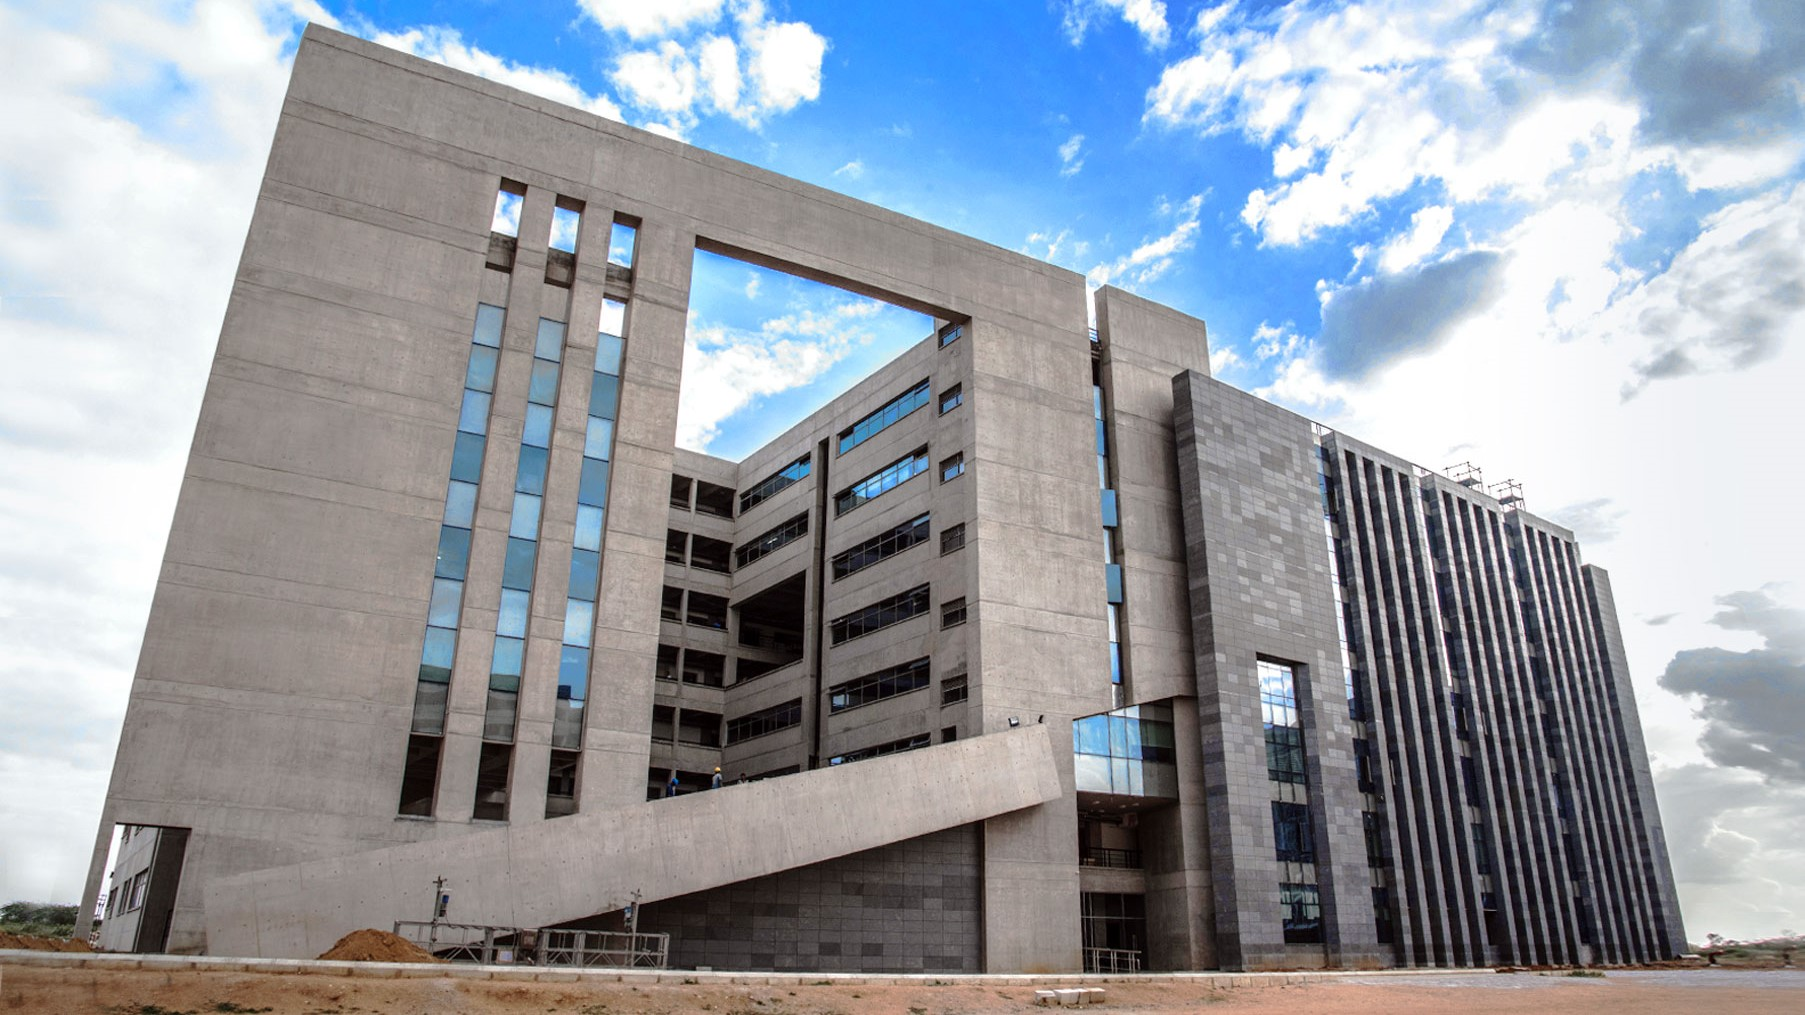
\includegraphics[height=\paperheight,width=\paperwidth]{IITH.jpg}};
}
\logo{
\includegraphics[height=1cm]{logo.png}}


\title[EE3025 - DSP Lab ]{Fast Fourier transform}
\subtitle{EE3025 - DSP Lab }
\author[K Srikanth]{K Srikanth - EE18BTECH11023}
\institute[IITH]{Indian Institute of Technology Hyderabad}
\date{\today}


\begin{document}
{\fontfamily{cmr}\selectfont
\begin{frame}
 \maketitle
 
\end{frame}

% \begin{frame}
% \frametitle{Table of Contents}
%  \tableofcontents
% \end{frame}


\section{Question} 
\begin{frame}{Question}
\begin{itemize}
        \item Let \[ x(n) = \{\underset{\uparrow}{1},2,3,4,2,1 \} \]\\
            \[ h(n)=\left(-\frac{1}{2}\right)^{n} u(n)+\left(-\frac{1}{2}\right)^{n-2} u(n-2)\]
        \item Compute X(k), H(k) and y(n) using FFT and IFFT 
        \item Wherever possible, express all the above equa-tions as matrix equations.
\end{itemize}

\end{frame}

\section{Solution }
\begin{frame}{Computing X(k), H(k) Using  FFT   }
 
\begin{itemize}
\item input signal x(n)
    \[ x(n) = \{ \underset{\uparrow}{1},2,3,4,2,1 \}\]
    \item Impulse Response of the System is
    \[h(n)=\left(-\frac{1}{2}\right)^{n} u(n)+\left(-\frac{1}{2}\right)^{n-2} u(n-2)\]
    \item FFT of a Input Signal $x(n)$ is 
     \[  X(k) = \sum_{n=0}^{N-1} x(n) e^{-j 2 \pi k n / N}, \quad k=0,1 \ldots N-1\]
    \item FFT of a Impulse Response $h(n)$ is 
    \[  H(k) = \sum_{n=0}^{N-1} h(n) e^{-j 2 \pi k n / N}, \quad k=0,1, \ldots, N-1\]
\end{itemize}

\end{frame} 
\begin{frame}{Plots of Magnitude and Phase of  X(k) and H(k) }
\begin{figure}
    \centering
    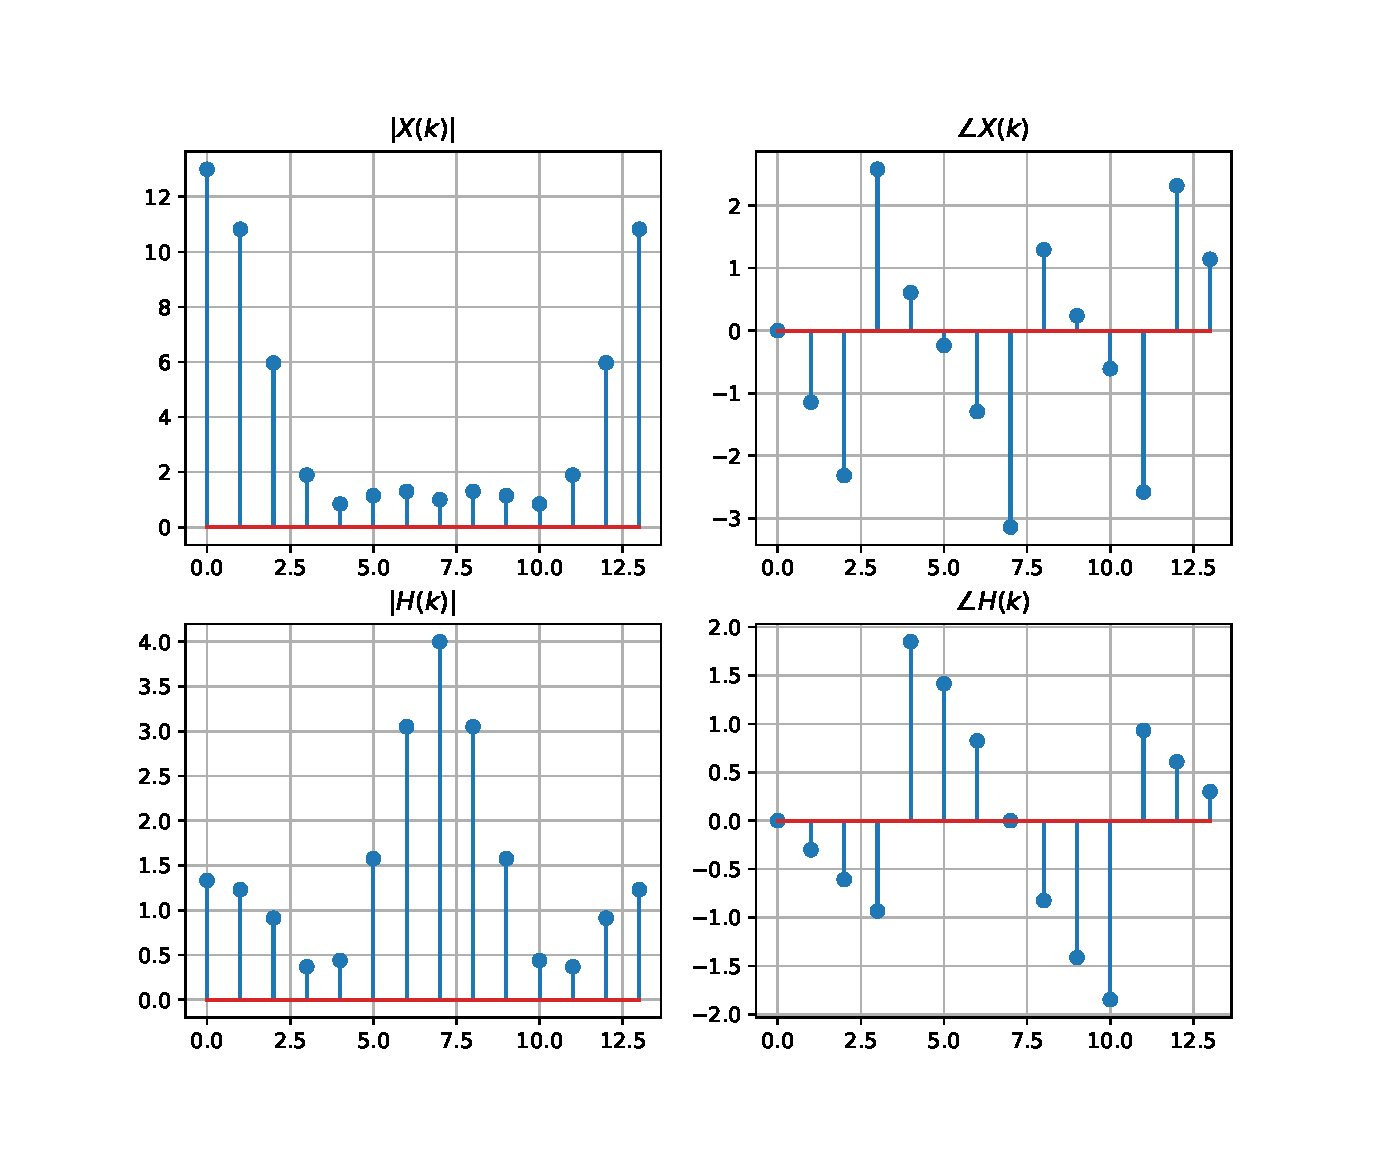
\includegraphics[width=8cm]{XH_fft.eps}
\end{figure}

\end{frame} 
\begin{frame}{Filter Output Using FFT and IFFT}
\begin{itemize}
    \item $y(n)$ can be computed by doing IFFT for $Y(k)$
    \[y(n) = \frac{1}{N}\sum_{n=0}^{N-1}Y(k) e^{j 2 \pi n k / N}, \quad k=0,1, \ldots, N-1\]
\end{itemize}
\begin{figure}
    \centering
    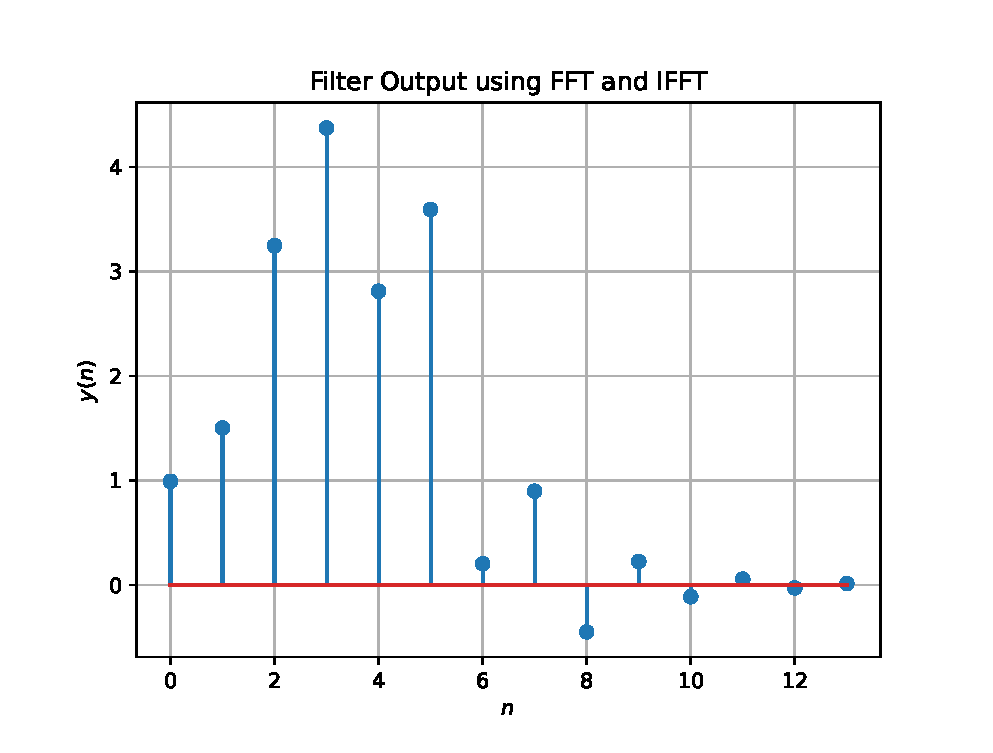
\includegraphics[width=6cm]{y_n.eps}
\end{figure}
\end{frame}

\section{Matrix Equations}
\begin{frame}{expressing all the above equations as matrix equations}
\begin{itemize}
       \item FFT of signal X(n) 
   \[
        X(k) \triangleq \sum_{n=0}^{N-1} x(n) e^{-j 2 \pi k n / N}, \quad k=0,1, \ldots, N-1
    \]
    \item Let $W_{N}^{n k}=e^{-j 2 \pi k n / N}$ then this can be $\mathrm{ex}-$ pressed interms of matrices as:
    
       \[ \begin{bmatrix} X(0) \\ X(1) \\ X(2) \\ X(3) \\ X(4) \\ X(5) \end{bmatrix}
=
\begin{bmatrix}
1 & 1 & 1 & 1 & 1 & 1 \\ 1 & W_N^1& W_N^2& W_N^3 & W_N^4 & W_N^5\\1 & W_N^2 & W_N^4 & W_N^6 & W_N^8 & W_N^{10}\\1 & W_N^3 & W_N^6 & W_N^9 & W_N^{12} & W_N^{15}\\1 & W_N^4 & W_N^8 & W_N^{12} & W_N^{16} & W_N^{20}\\1 & W_N^5 & W_N^{10} & W_N^{15} & W_N^{20} &W_N^{25}
\end{bmatrix}\begin{bmatrix}
x(0) \\ x(1) \\ x(2) \\ x(3) \\ x(4) \\x(5)
\end{bmatrix}\]
\end{itemize}



\end{frame}
 \begin{frame}{Computing X(K) from Matrix Equations}
  \begin{itemize}
      \item
On solving we get,
\[\implies X(0) = 13 + 0j,\]
\[X(1) = -4 - 1.732j,\]
\[X(2) = 1 + 0j\]
\[X(3) = -1 + 0j,\]
\[X(4) = 1 + 0j,\]
\[X(5) = -4 + 1.732j\]
\item the impluse
\[
 h(n)=\frac{-1}{2}^nu(n) + \frac{-1}{2}^{n-2}u(n-2)
\]
assuming that length of h(n) is same as length of x(n) i.e., N = 6.\\
Similarly like x(n), solving h(n) using matrix method for each value of k we get,
  \end{itemize}  
\end{frame}

\begin{frame}{Computing H(K) from Matrix Equations}

       \[
    \begin{bmatrix} H(0) \\ H(1) \\ H(2) \\ H(3) \\ H(4) \\ H(5) \end{bmatrix}
=
\begin{bmatrix}
h(0) + h(1) + h(2) + h(3) + h(4) + h(5) \\h(0) + h(1)e^{-j\pi /3} + ... + h(5)e^{-j5\pi /3}\\h(0) + h(1)e^{-2j\pi /3} + ... + h(5)e^{-2j5\pi /3}\\h(0) + h(1)e^{-3j\pi /3} + ... + h(5)e^{-3j5\pi /3}\\
h(0) + h(1)e^{-4j\pi /3} + ... + h(5)e^{-4j5\pi /3}\\h(0) + h(1)e^{-5j\pi /3} + ... + h(5)e^{-5j5\pi /3}
\end{bmatrix}
\]
 On solving we get\\
H(0) = 1.28125 + 0j \;,
H(1) = 0.51625 - 0.5141875j \; ,\\
H(2) = -0.078125 + 1.1095625j \;,
H(3) = 3.84375 + 0j \;,\\
H(4) = -0.071825 - 1.1095625j \;,
H(5) = 0.515625 + 0.5141875j

\end{frame}

\begin{frame}{Computing Y(K) from Matrix Equations}
We can now compute Y(k) using below equation
   \[ Y(k) = X(k)H(k)\]
So, Y(k) is obtained element wise multiplication of X(k) and H(k)
\[\begin{bmatrix} 
Y(0) \\ Y(1) \\ Y(2) \\ Y(3) \\ Y(4) \\ Y(5) 
\end{bmatrix}
=
\begin{bmatrix}
X(0)\cdot H(0) \\ X(1)\cdot H(1) \\ X(2)\cdot H(2) \\ X(3)\cdot H(3) \\ X(4)\cdot H(4) \\ X(5)\cdot H(5)
\end{bmatrix}\]

Computing the above expression we get,
 \[
\begin{bmatrix} 
Y(0) \\ Y(1) \\ Y(2) \\ Y(3) \\ Y(4) \\ Y(5) 
\end{bmatrix}
=
\begin{bmatrix}
16.6562+0j \\ -2.95312+1.16372j \\ -0.07812+1.10959j \\ -3.84375-9.27556j \\ -0.07812-1.10959j \\ -2.95312-1.16372j 
\end{bmatrix}\]


\end{frame}
\begin{frame}{Computinh y(n) from IFFT of Y matrix}
   
y(n) is given by IFFT of Y matrix. this y(n) can be calculated by a python code 

\[
    \begin{bmatrix} 
y(0) \\ y(1) \\ y(2) \\ y(3) \\ y(4) \\ y(5) 
\end{bmatrix}
=
\begin{bmatrix}
1.125     +0j \\ 2.28125071+0j \\ 2.6250019 -1.11022302 \times 10^{-16}j \\ 4.37499667-1.47104551\times 10^{-15}j \\ 2.6562481 +6.10622664 \times 10^{-16}j \\ 3.59375262-1.60982339 \times 10^{-15}j 
\end{bmatrix}
\]
\end{frame}
}
\end{document}
